\documentclass[tikz,border=14pt]{standalone}
\usepackage[utf8]{inputenc}
\usepackage[T1]{fontenc}
\usepackage{lmodern}
\usepackage{amsmath}
\usetikzlibrary{arrows.meta,positioning,shapes.geometric,fit,backgrounds}

\definecolor{navy}{RGB}{24,58,92}
\definecolor{navyfill}{RGB}{236,243,250}
\definecolor{teal}{RGB}{15,118,110}
\definecolor{tealfill}{RGB}{234,248,246}
\definecolor{amber}{RGB}{180,83,9}
\definecolor{amberfill}{RGB}{254,245,231}
\definecolor{greenborder}{RGB}{27,94,32}
\definecolor{greenfill}{RGB}{235,247,237}
\definecolor{slate}{RGB}{71,85,105}
\definecolor{boxbg}{RGB}{248,250,252}

\begin{document}
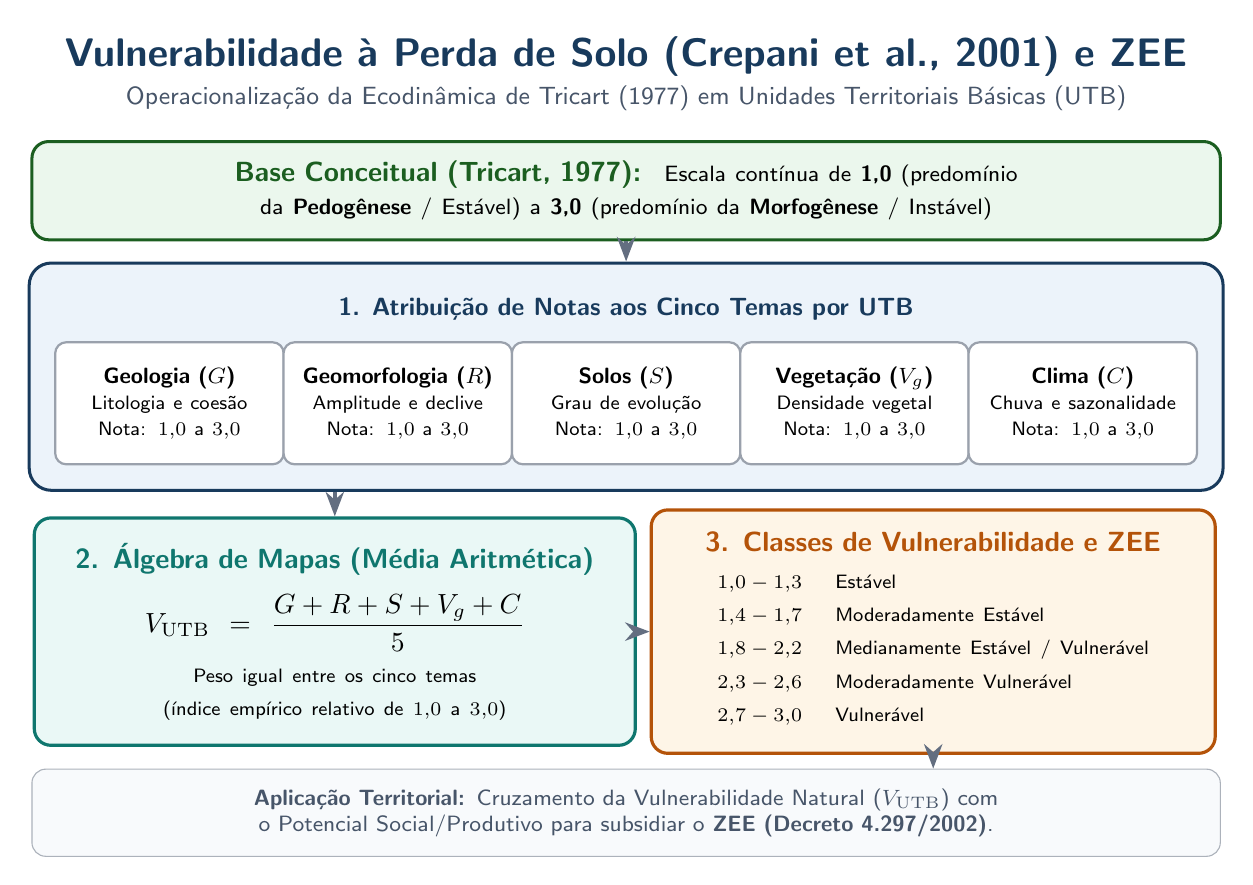
\begin{tikzpicture}[
  font=\sffamily,
  >=Stealth,
  title/.style={font=\sffamily\bfseries\Large, text=navy},
  subtitle/.style={font=\sffamily\small, text=slate},
  subbox/.style={
    rectangle, rounded corners=4pt, draw=slate!55, line width=0.8pt,
    fill=white, align=center, inner sep=5pt, font=\sffamily\footnotesize,
    minimum height=1.55cm
  },
  arrow/.style={->, line width=1.3pt, color=slate!85}
]

% Cabeçalho
\node[title] (hdr) at (0, 5.55) {Vulnerabilidade à Perda de Solo (Crepani et al., 2001) e ZEE};
\node[subtitle] at (0, 5.02) {Operacionalização da Ecodinâmica de Tricart (1977) em Unidades Territoriais Básicas (UTB)};

% Base Tricart
\node[rectangle, rounded corners=6pt, draw=greenborder, line width=1.1pt, fill=greenfill,
      text width=14.6cm, align=center, inner sep=7pt] (base) at (0, 3.85) {
  \textbf{\color{greenborder}Base Conceitual (Tricart, 1977):} \
  {\footnotesize Escala contínua de \textbf{1,0} (predomínio da \textbf{Pedogênese} / Estável) a \textbf{3,0} (predomínio da \textbf{Morfogênese} / Instável)}
};

% 5 Temas com título interno ao grupo
\node[font=\sffamily\bfseries\small, text=navy] (lbl1) at (0, 2.35) {1. Atribuição de Notas aos Cinco Temas por UTB};
\node[subbox, text width=2.55cm] (g) at (-5.8, 1.15) {\textbf{Geologia ($G$)}\\{\scriptsize Litologia e coesão}\\{\scriptsize Nota: $1{,}0$ a $3{,}0$}};
\node[subbox, text width=2.55cm] (r) at (-2.9, 1.15) {\textbf{Geomorfologia ($R$)}\\{\scriptsize Amplitude e declive}\\{\scriptsize Nota: $1{,}0$ a $3{,}0$}};
\node[subbox, text width=2.55cm] (s) at (0.0, 1.15) {\textbf{Solos ($S$)}\\{\scriptsize Grau de evolução}\\{\scriptsize Nota: $1{,}0$ a $3{,}0$}};
\node[subbox, text width=2.55cm] (vg) at (2.9, 1.15) {\textbf{Vegetação ($V_g$)}\\{\scriptsize Densidade vegetal}\\{\scriptsize Nota: $1{,}0$ a $3{,}0$}};
\node[subbox, text width=2.55cm] (c) at (5.8, 1.15) {\textbf{Clima ($C$)}\\{\scriptsize Chuva e sazonalidade}\\{\scriptsize Nota: $1{,}0$ a $3{,}0$}};

\begin{scope}[on background layer]
  \node[rectangle, rounded corners=8pt, draw=navy, line width=1.1pt, fill=navyfill,
        fit=(lbl1)(g)(r)(s)(vg)(c), inner sep=9pt] (grp1) {};
\end{scope}

% Equação
\node[rectangle, rounded corners=6pt, draw=teal, line width=1.15pt, fill=tealfill,
      text width=7.0cm, align=center, inner sep=9pt, minimum height=2.7cm] (calc) at (-3.7, -1.75) {
  \textbf{\color{teal}2. Álgebra de Mapas (Média Aritmética)}\\[6pt]
  {\normalsize $V_{\mathrm{UTB}} = \dfrac{G + R + S + V_g + C}{5}$}\\[6pt]
  {\scriptsize Peso igual entre os cinco temas (índice empírico relativo de $1{,}0$ a $3{,}0$)}
};

% Classificação
\node[rectangle, rounded corners=6pt, draw=amber, line width=1.15pt, fill=amberfill,
      text width=6.6cm, align=center, inner sep=8pt, minimum height=2.7cm] (cls) at (3.9, -1.75) {
  \textbf{\color{amber}3. Classes de Vulnerabilidade e ZEE}\\[4pt]
  \begin{tabular}{@{}ll@{}}
    {\scriptsize $1{,}0 - 1{,}3$} & {\scriptsize Estável} \\
    {\scriptsize $1{,}4 - 1{,}7$} & {\scriptsize Moderadamente Estável} \\
    {\scriptsize $1{,}8 - 2{,}2$} & {\scriptsize Medianamente Estável / Vulnerável} \\
    {\scriptsize $2{,}3 - 2{,}6$} & {\scriptsize Moderadamente Vulnerável} \\
    {\scriptsize $2{,}7 - 3{,}0$} & {\scriptsize Vulnerável} \\
  \end{tabular}
};

% Rodapé
\node[rectangle, rounded corners=5pt, draw=slate!45, fill=boxbg, text width=14.6cm,
      align=center, inner sep=7pt, font=\sffamily\footnotesize, text=slate] (rod) at (0, -4.05) {
  \textbf{Aplicação Territorial:} Cruzamento da Vulnerabilidade Natural ($V_{\mathrm{UTB}}$) com o Potencial Social/Produtivo para subsidiar o \textbf{ZEE (Decreto 4.297/2002)}.
};

% Setas limpas sem cruzar textos
\draw[arrow] (base.south) -- (grp1.north);
\draw[arrow] (grp1.south -| calc.north) -- (calc.north);
\draw[arrow] (calc.east) -- (cls.west);
\draw[arrow] (cls.south) -- (cls.south |- rod.north);

\end{tikzpicture}
\end{document}
